\documentclass[12pt, titlepage]{article}

\usepackage{booktabs}
\usepackage{tabularx}
\usepackage{graphicx}
\usepackage{hyperref}
\hypersetup{
    colorlinks,
    citecolor=black,
    filecolor=black,
    linkcolor=red,
    urlcolor=blue
}
\usepackage[round]{natbib}

%% Comments

\usepackage{color}

\newif\ifcomments\commentstrue

\ifcomments
\newcommand{\authornote}[3]{\textcolor{#1}{[#3 ---#2]}}
\newcommand{\todo}[1]{\textcolor{red}{[TODO: #1]}}
\else
\newcommand{\authornote}[3]{}
\newcommand{\todo}[1]{}
\fi

\newcommand{\wss}[1]{\authornote{blue}{SS}{#1}} 
\newcommand{\plt}[1]{\authornote{magenta}{TPLT}{#1}} %For explanation of the template
\newcommand{\an}[1]{\authornote{cyan}{Author}{#1}}


\begin{document}

\title{Test Report: Lights, Camera, Models!} 
\author{Sasha Soraine}
\date{\today}
	
\maketitle

\pagenumbering{roman}

\section{Revision History}

\begin{tabularx}{\textwidth}{p{3cm}p{2cm}X}
\toprule {\bf Date} & {\bf Version} & {\bf Notes}\\
\midrule
December 18, 2019 & 1.0 & Original Version.\\
\bottomrule
\end{tabularx}

~\newpage

\section{Symbols, Abbreviations and Acronyms}

\renewcommand{\arraystretch}{1.2}
\begin{tabular}{l l} 
  \toprule		
  \textbf{symbol} & \textbf{description}\\
  \midrule 
  T & Test\\
  \bottomrule
\end{tabular}\\

\wss{symbols, abbreviations or acronyms -- you can reference the SRS tables if needed}

\newpage

\tableofcontents

\listoftables %if appropriate

\listoffigures %if appropriate

\newpage

\pagenumbering{arabic}

This document is the System and Unit VnV Test Report for Lights, Camera, Models!
Due to limitations with time, and the extensive use of Unity's built-in modules 
which were assumed to function correctly, this report will predominantly 
feature the manual testing outlined in System VnV.

\section{Functional Requirements Evaluation}
\sms{I am unsure how to write about this evaluation given that all of my tests 
are manually comparing scene renders.}

\subsubsection{Run-Time Tests}
All of these test cases share the following properties:
\begin{itemize}
	\item[] Initial State: Lighting Model = Lambert\\
	ks = 0.5 \\ kd = 1 \\ $\alpha$ = 1 \\ Colour = () \\ Specular Colour = 
	White \\ Light Type = Spotlight \\ Light Colour = White \\ 
\end{itemize}

This means the default scene should look like this:

\begin{figure}
	\centering
	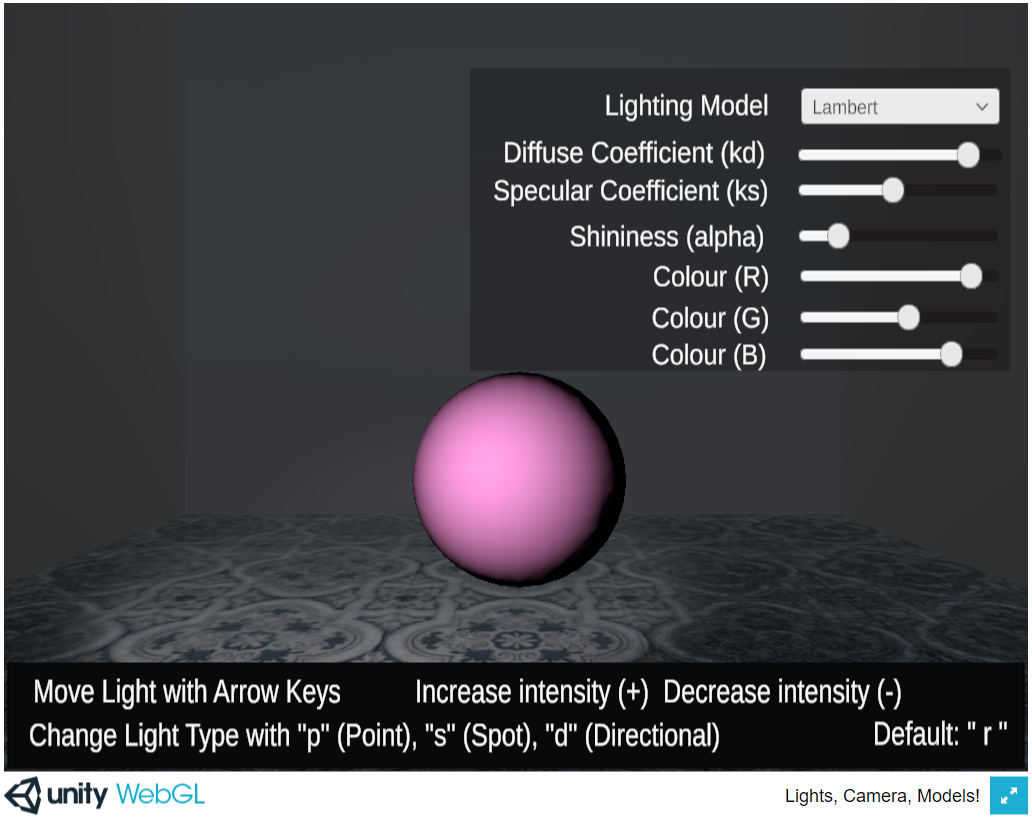
\includegraphics[scale=0.25]{./images/fromVnVPlan/sphere-lit-lambert}
	\caption{Expected: Default Scene}
\end{figure}

Our finished default scene looks like this:
\begin{figure}
	\centering
	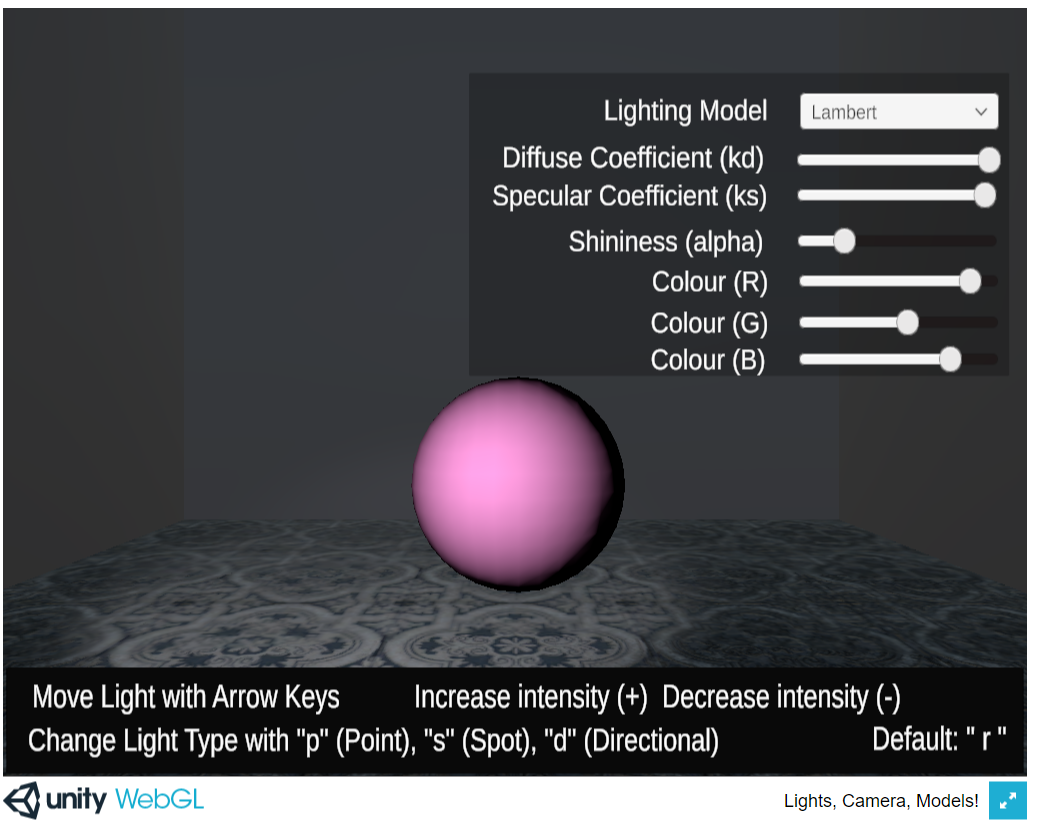
\includegraphics[scale=0.25]{./images/defaultScene-final}
	\caption{Actual: Default Scene for Lights, Camera, Models!}
\end{figure}

~\newline
\paragraph{Lighting Model Changes}

\begin{enumerate}
	
	\item{lightModel-ModLambert\\}
	
	Control: Manual
	
	Input: Select Mod-Lambert lighting model from dropdown list.
	
	Output: Scene render with Mod-Lambert lit sphere.
	
	\begin{figure}[h]
		\centering
		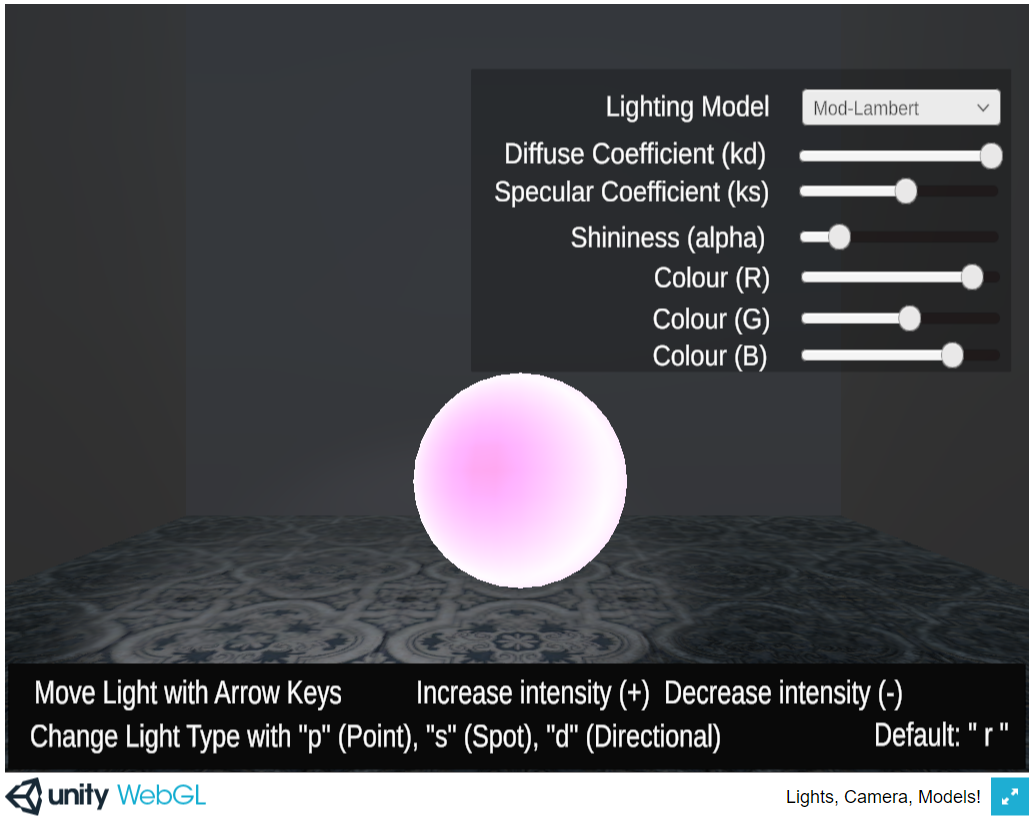
\includegraphics[scale=0.25]{./images/fromVnVPlan/sphere-lit-modlambert}
		\caption{Expected Output: Default Scene with Lighting Model changed to 
		Mod-Lambert}
		\label{fig:modLambert}
	\end{figure}
	
	\begin{figure}
		\centering
		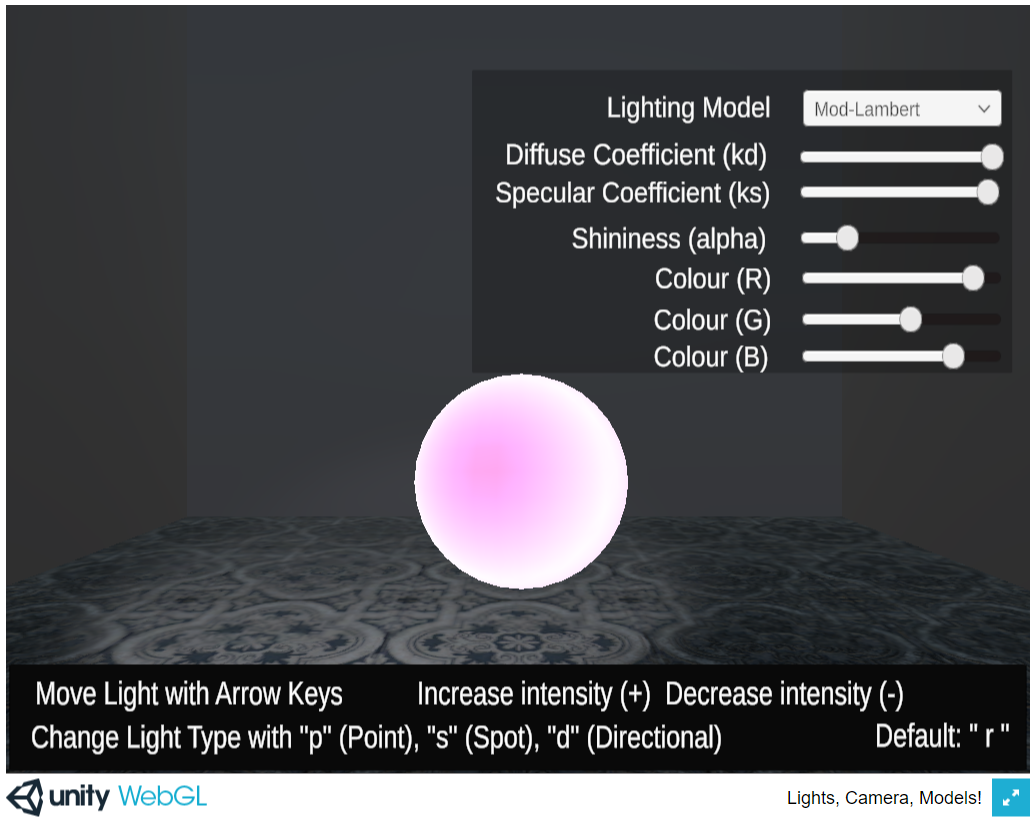
\includegraphics[scale=0.25]{./images/defaultScene-mLam}
		\caption{Actual: Default Scene for Lights, Camera, Models! with 
		ModLambert}
	\end{figure}
	
	\item{lightModel-Phong\\}
	
	Control: Manual
	
	Input: Select Phong lighting model from dropdown list. 
	
	Output: Scene render with Phong lit sphere.
	
	\begin{figure}[h]
		\centering
		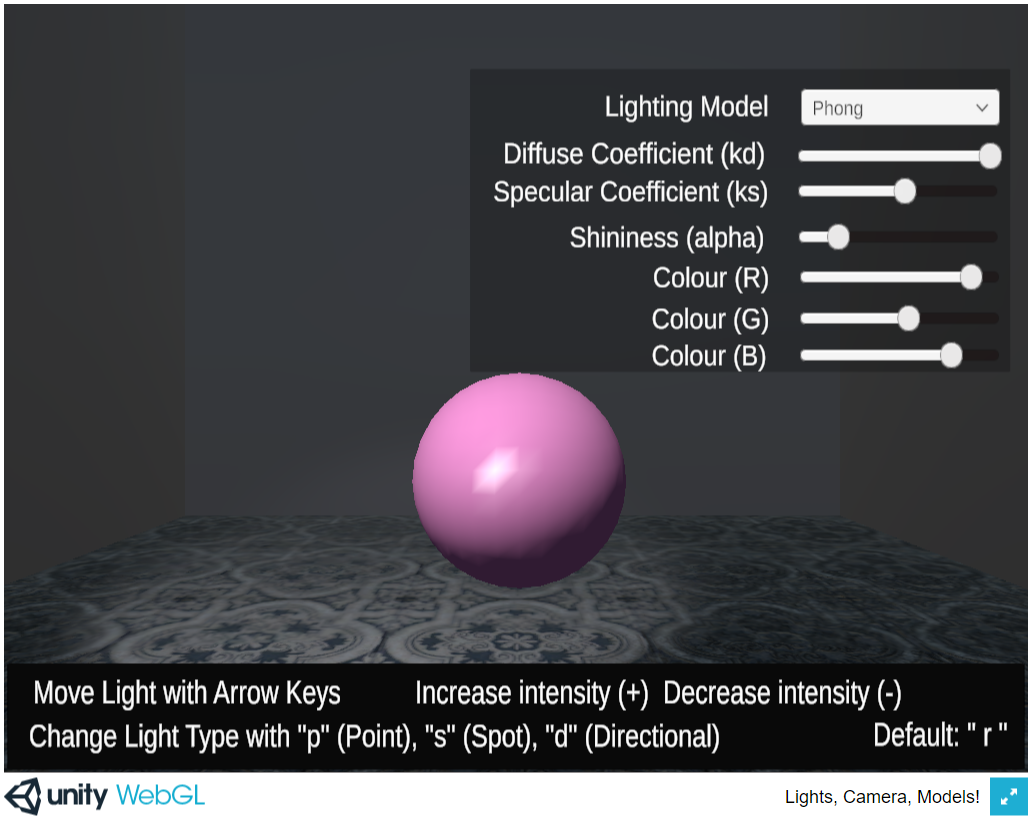
\includegraphics[scale=0.25]{./images/fromVnVPlan/sphere-lit-phong}
		\caption{Default Scene with Lighting Model changed to Phong}
		\label{fig:Phong}
	\end{figure}
	

	\item{lightModel-BlinnPhong\\}
	
	Control: Manual
	
	Input: Select Blinn-Phong lighting model from dropdown list. 
	
	Output: Scene render with Blinn-Phong lit sphere.
	
	\begin{figure}[h]
		\centering
		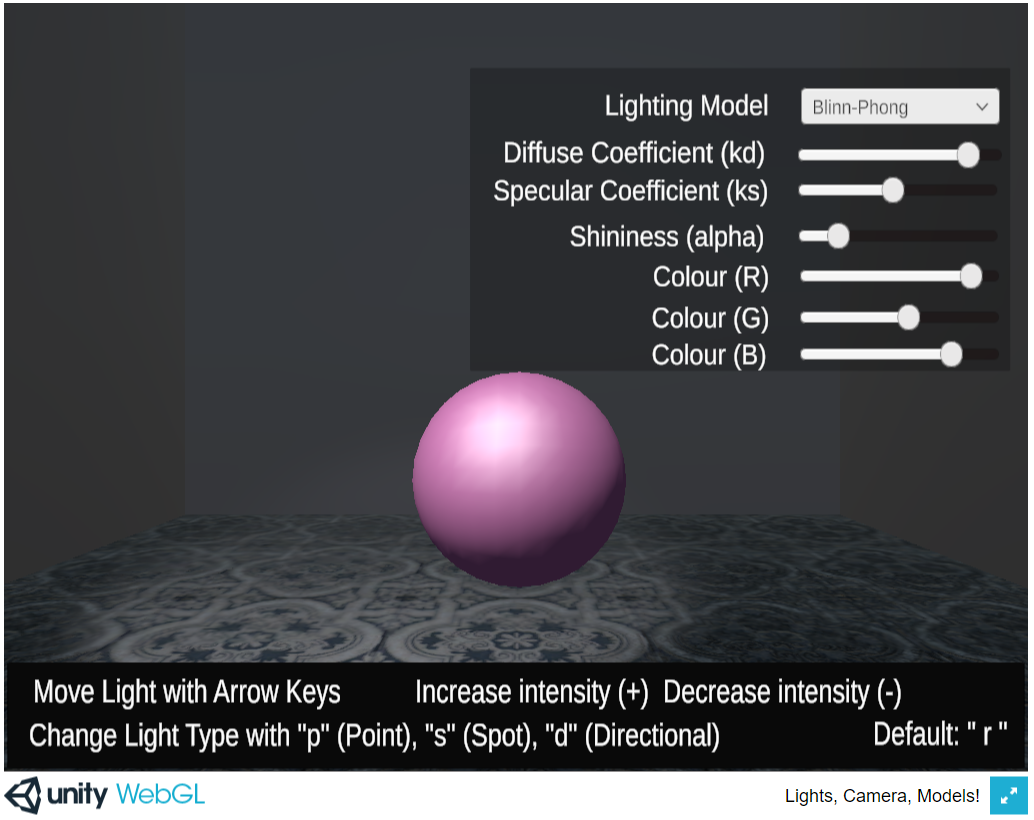
\includegraphics[scale=0.25]{./images/fromVnVPlan/sphere-lit-blinnphong}
		\caption{Default Scene with Lighting Model changed to Blinn-Phong}
		\label{fig:blinnPhong}
	\end{figure}
	
	
\end{enumerate}

\paragraph{Object Changes}

\begin{enumerate}
	%%Object Material Properties
	%Valid changes	
	\item{objMaterialPropChange-valid-ks\\}
	
	Control: Manual
	
	Initial State: Default Scene with lighting model set to Blinn-Phong (see 
	\ref{fig:blinnPhong})
	
	Input: $k_{s} = 1$
	
	Output: Scene render with Blinn-Phong lit and brighter and larger specular 
	reflection.
	
	\begin{figure}[h]
		\centering
		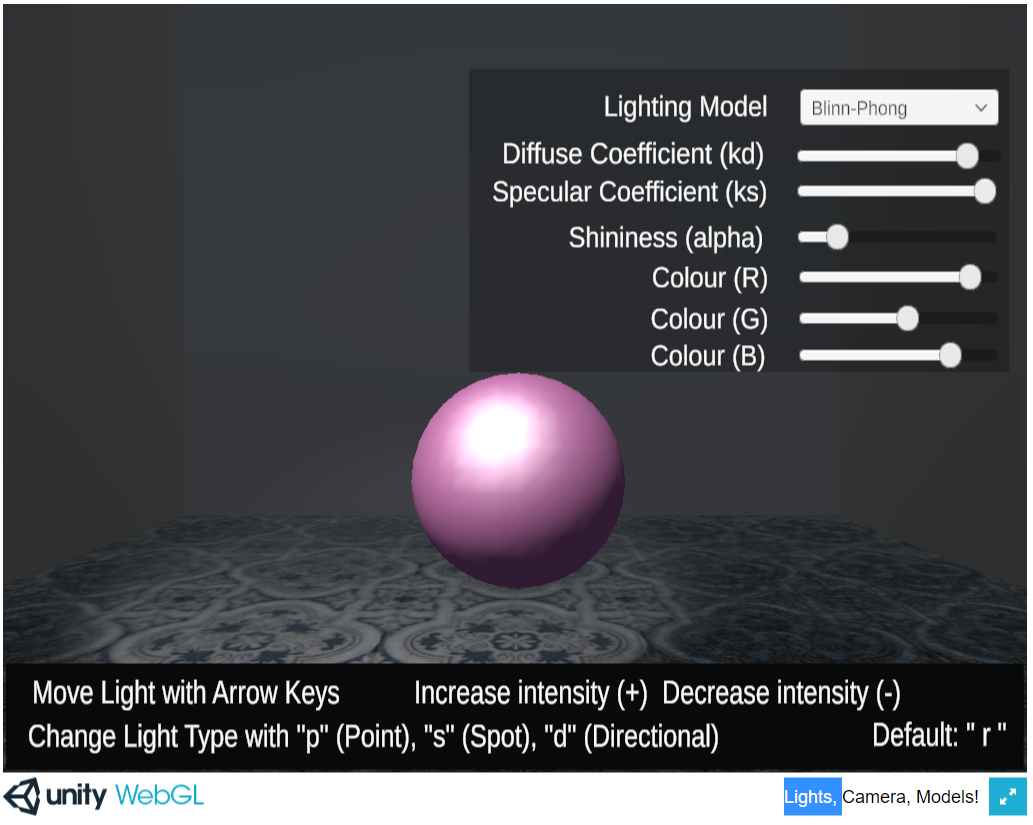
\includegraphics[scale=0.25]{./images/fromVnVPlan/sphere-lit-blinnphong-ks1}
		\caption{Default Scene with Lighting Model changed to Blinn-Phong and 
			$k_{s}$ set to 1}
		\label{fig:blinnPhong-ks1}
	\end{figure}
	
	
	
	\item{objMaterialPropChange-valid-kd\\}
	
	Control: Manual
	
	Input: $k_{d} = 0.5$
	
	Output: Scene render with Blinn-Phong lit, with colour of sphere being dull.
	\begin{figure}[h]
		\centering
		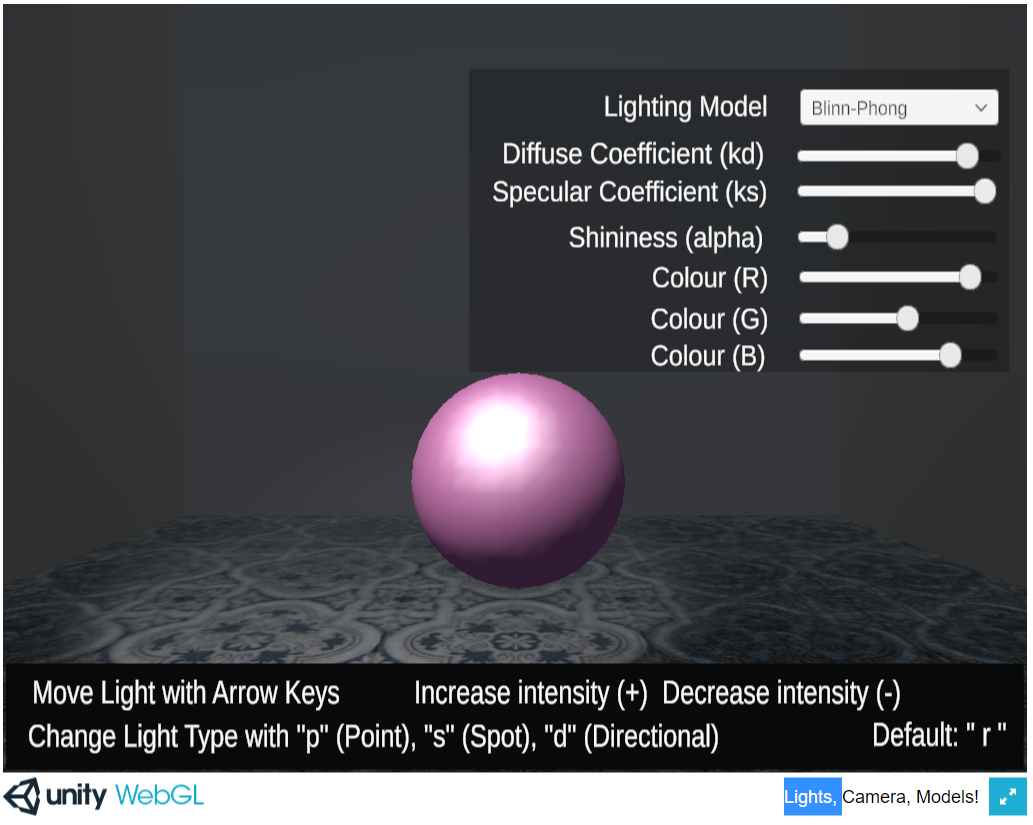
\includegraphics[scale=0.25]{./images/fromVnVPlan/sphere-lit-blinnphong-ks1}
		\caption{Default Scene with Lighting Model changed to Blinn-Phong and 
			$k_{s}$ set to 1}
		\label{fig:blinnPhong-kd0.5}
	\end{figure}	
	
	


	\item{objMaterialPropChange-valid-$\alpha$\\}
	
	Control: Manual
	
	Input: $\alpha = 100$
	
	Output: Scene render of Blinn-Phong lit sphere and smaller sharper specular 
	reflection.
	\begin{figure}[h]
		\centering
		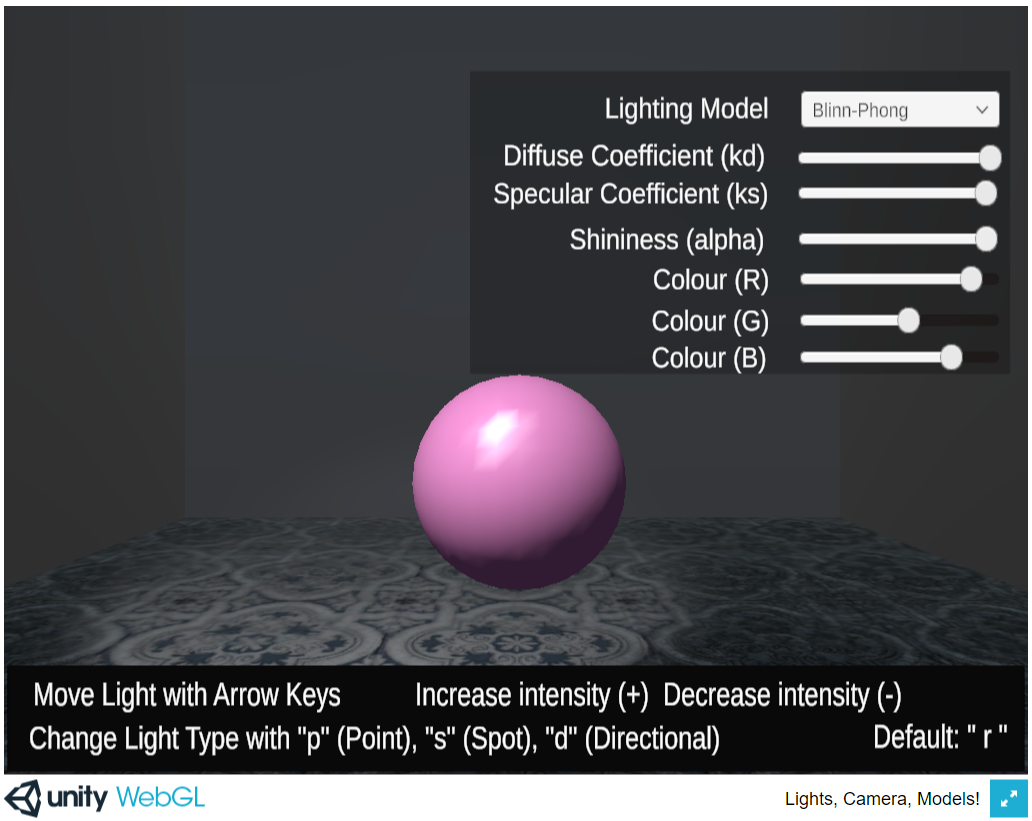
\includegraphics[scale=0.25]{./images/fromVnVPlan/sphere-lit-blinnphong-a100}
		\caption{Default Scene with Lighting Model changed to Blinn-Phong and 
			$\alpha$ set to 100}
		\label{fig:blinnPhong-a100}
	\end{figure}		
	
	
	
	%%Object Colour
	\item{objColour-valid-base\\}
	
	Control: Automatic
	
	Input: New (r,g,b) value for BASE\_COLOUR picked from GUI picker = 
	(0,0,0).
	
	Output: Scene render of Blinn-Phong with a black object material. All 
	diffuse terms need to be recalculated.
	
	\begin{figure}[h]
		\centering
		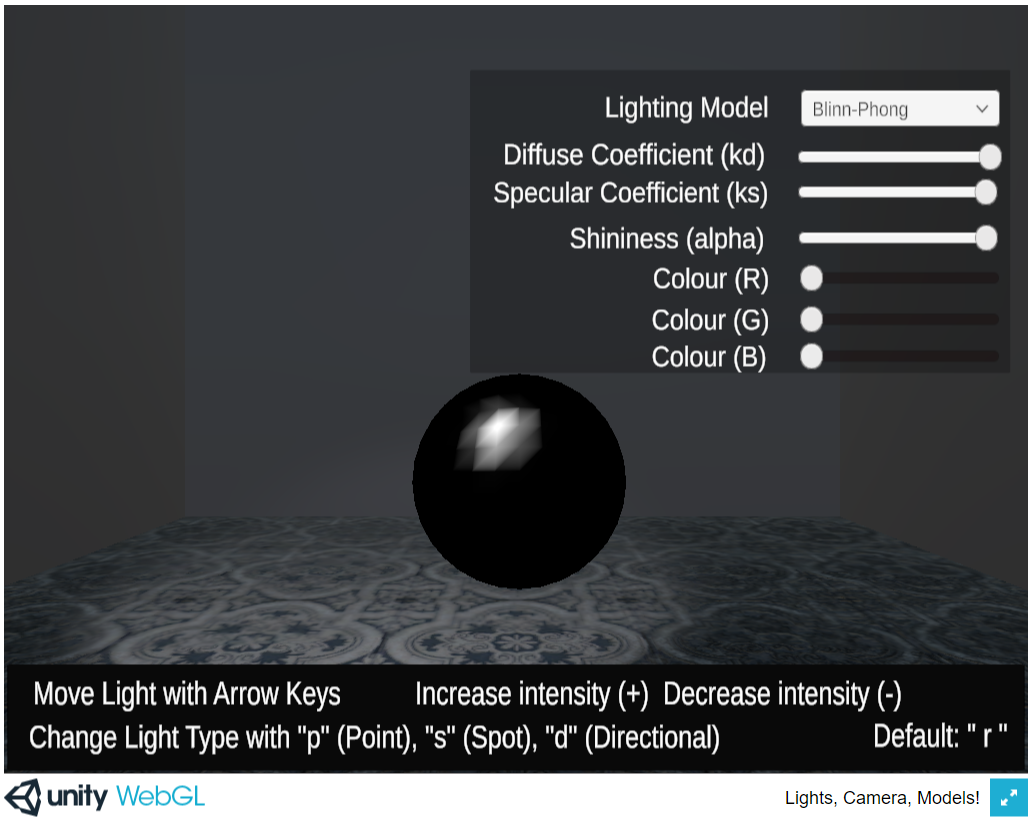
\includegraphics[scale=0.25]{./images/fromVnVPlan/sphere-lit-blinnphong-colour}
		\caption{Default Scene with Lighting Model changed to Blinn-Phong and 
			BASE\_COLOUR set to (0,0,0)}
		\label{fig:blinnPhong-black}
	\end{figure}	
	


\end{enumerate}

\paragraph{Light Changes}

\begin{enumerate}
	%%Light Positions
	%Valid
	\item{lightPos-valid\\}
	
	Control: Manual
	
	Input: \\
	\textit{Variation 1}: Light Type = Spotlight, Press left arrow 5 times\\
	\textit{Variation 2}: Light Type = Point Light, Press left arrow key 5 
	times\\
	\textit{Variation 3}: Light Type = Directional, Press right arrow key 5 
	times\\
	\textit{Variation 4}: Light Type = Spotlight, Press right arrow key 10
	times\\
	\textit{Variation 5}: Light Type = Point Light, Press right arrow key 10
	times\\
	
	Output: Scene render based on new position of light source.
	
	\begin{figure}[h]
		\centering
		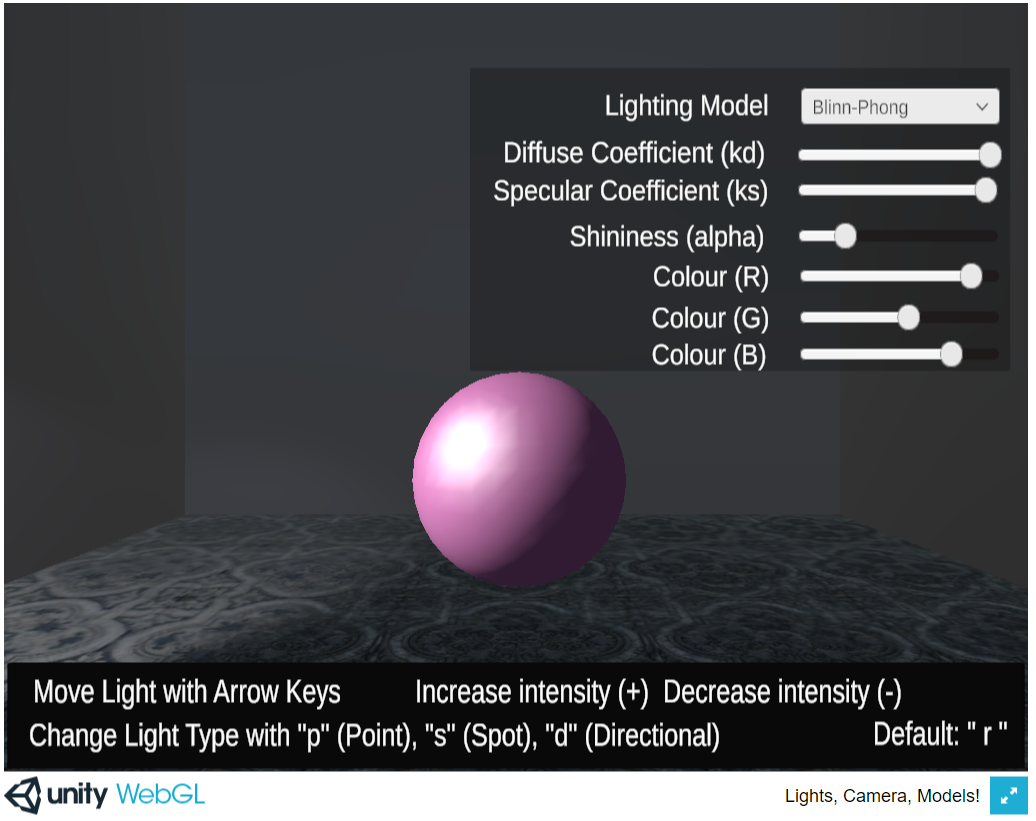
\includegraphics[scale=0.25]{./images/fromVnVPlan/sphere-lit-spotlight-moveValid}
		\caption{Output Variation 1}
		\label{fig:spotlight-move}
	\end{figure}	
	
	\begin{figure}[h]
		\centering
		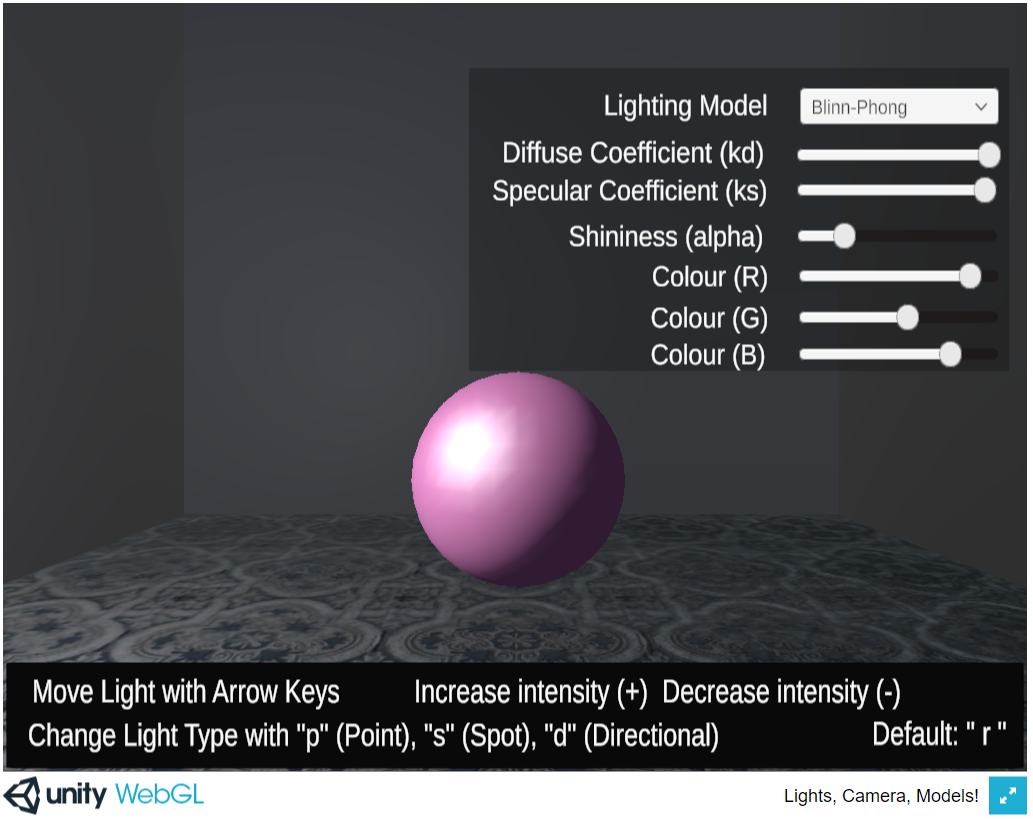
\includegraphics[scale=0.25]{./images/fromVnVPlan/sphere-lit-point-moveValid}
		\caption{Output Variation 2}
		\label{fig:point-move}
	\end{figure}	
	
	\begin{figure}[h]
		\centering
		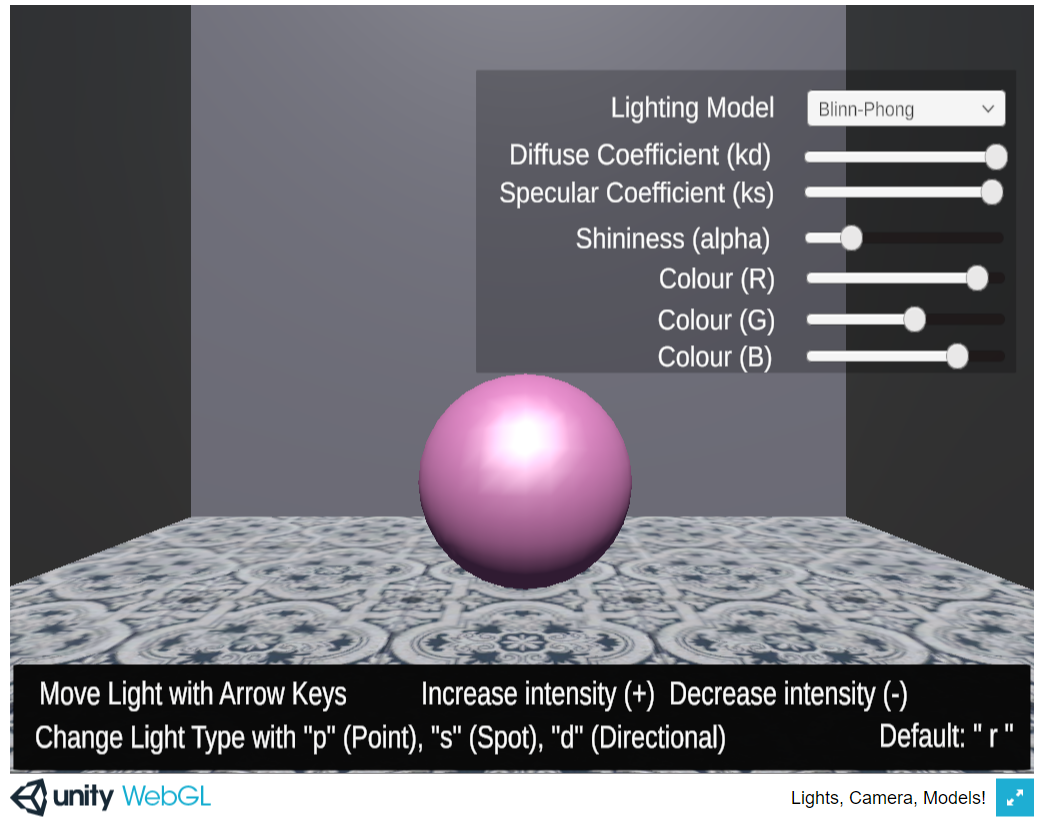
\includegraphics[scale=0.25]{./images/fromVnVPlan/sphere-lit-direction}
		\caption{Output Variation 3}
		\label{fig:directional-move}
	\end{figure}
	
	\begin{figure}[h]
		\centering
		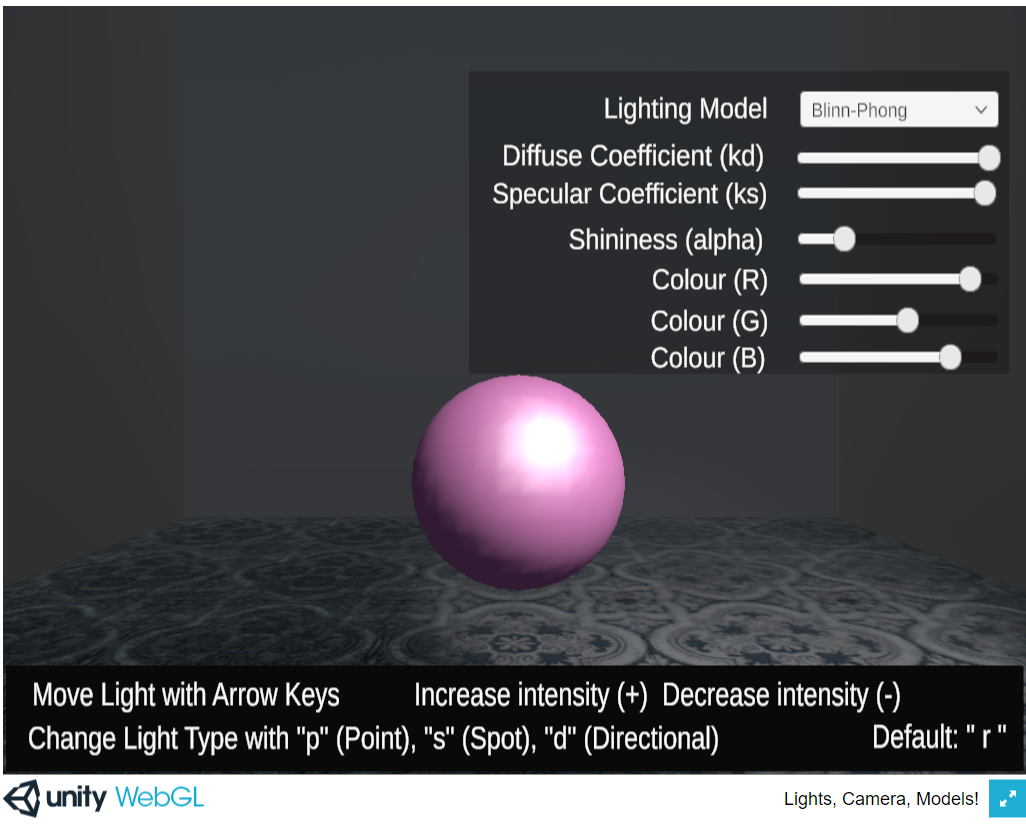
\includegraphics[scale=0.25]{./images/fromVnVPlan/sphere-lit-spotlight-moveValidR}
		\caption{Output Variation 4}
		\label{fig:spotlight-move-right}
	\end{figure}	
	
	\begin{figure}[h]
		\centering
		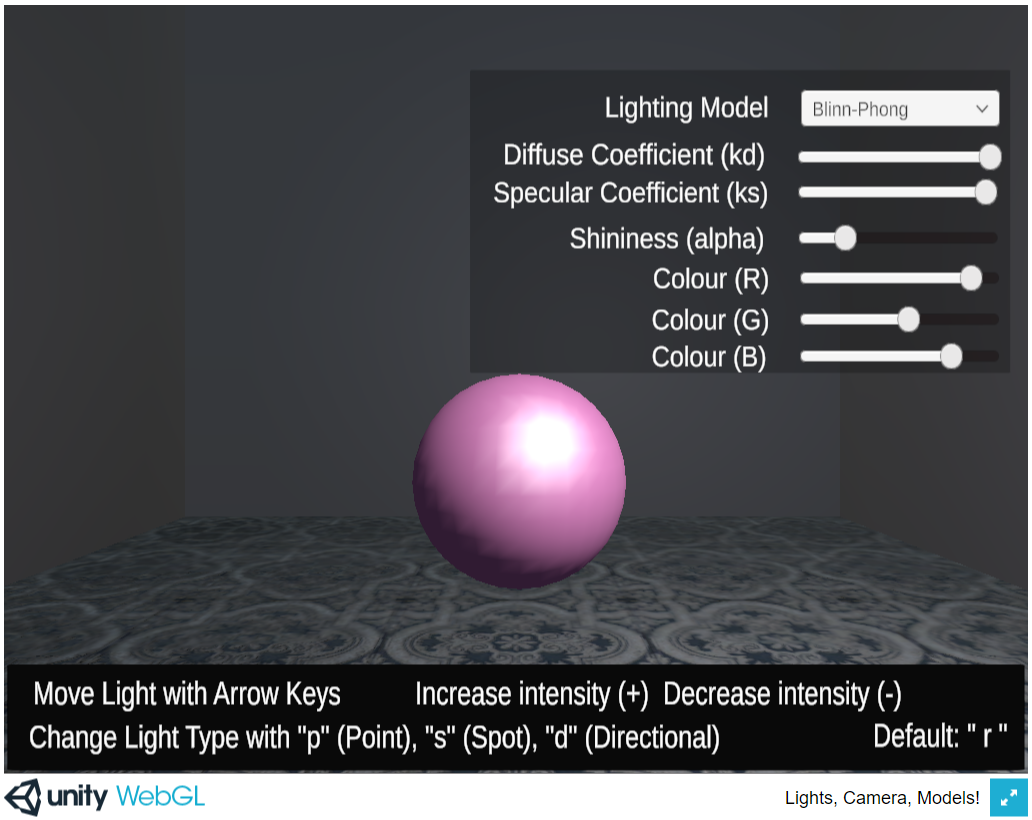
\includegraphics[scale=0.25]{./images/fromVnVPlan/sphere-lit-point-moveValidR}
		\caption{Output Variation 5}
		\label{fig:point-move-right}
	\end{figure}	
	
	

	\item{lightPos-boundaries\\}
	
	Control: Manual
	
	Input:  \\
	\textit{Variation 1}: Light Type = Spotlight, Press right arrow key 31 
	times\\
	\textit{Variation 2}: Light Type = Point Light, Press right arrow key 31 
	times\\
	\textit{Variation 3}: Light Type = Directional, Press right arrow key 31 
	times\\
	\textit{Variation 4}: Light Type = Spotlight, Press left arrow key 20 
	times\\
	\textit{Variation 5}: Light Type = Point Light, Press left arrow key 20 
	times\\
	
	Output: Scene render and lit with Blinn-Phong lighting model, and 
	reflections changing depending on the position of the light.
	
	\begin{figure}[h]
		\centering
		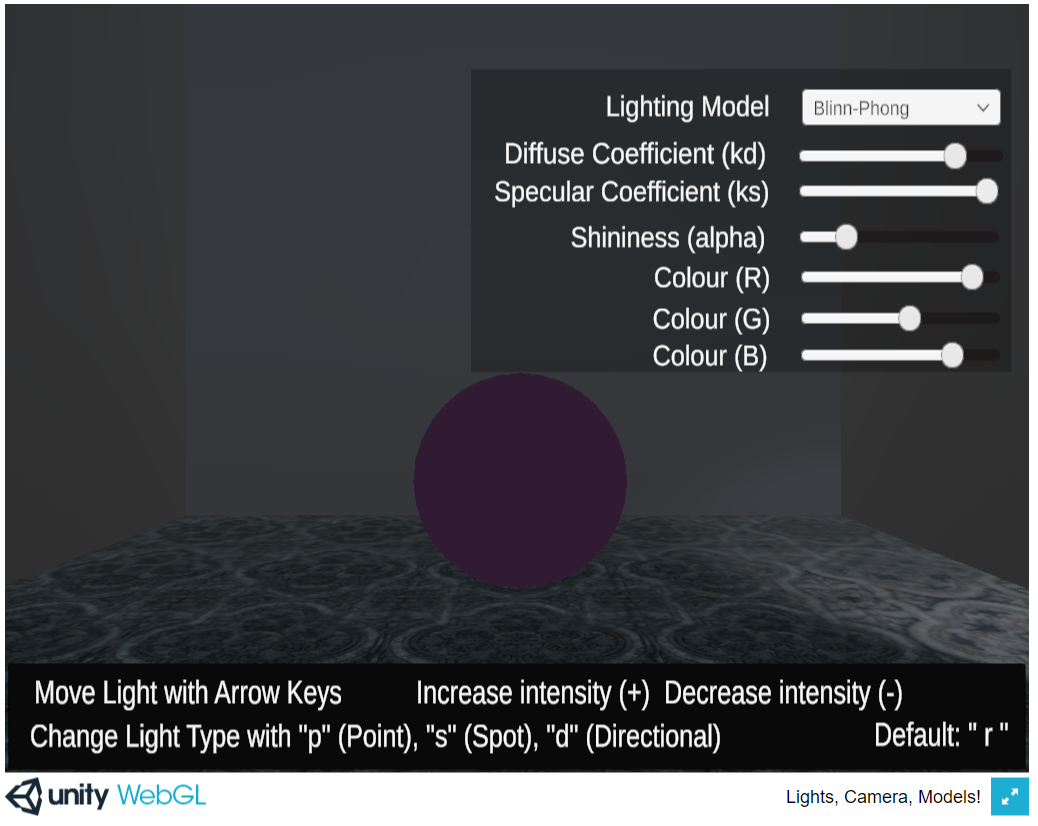
\includegraphics[scale=0.25]{./images/fromVnVPlan/sphere-lit-spotlight-moveBoundsR}
		\caption{Output Variation 1}
		\label{fig:spotlight-bounds-right}
	\end{figure}	
	
	\begin{figure}[h]
		\centering
		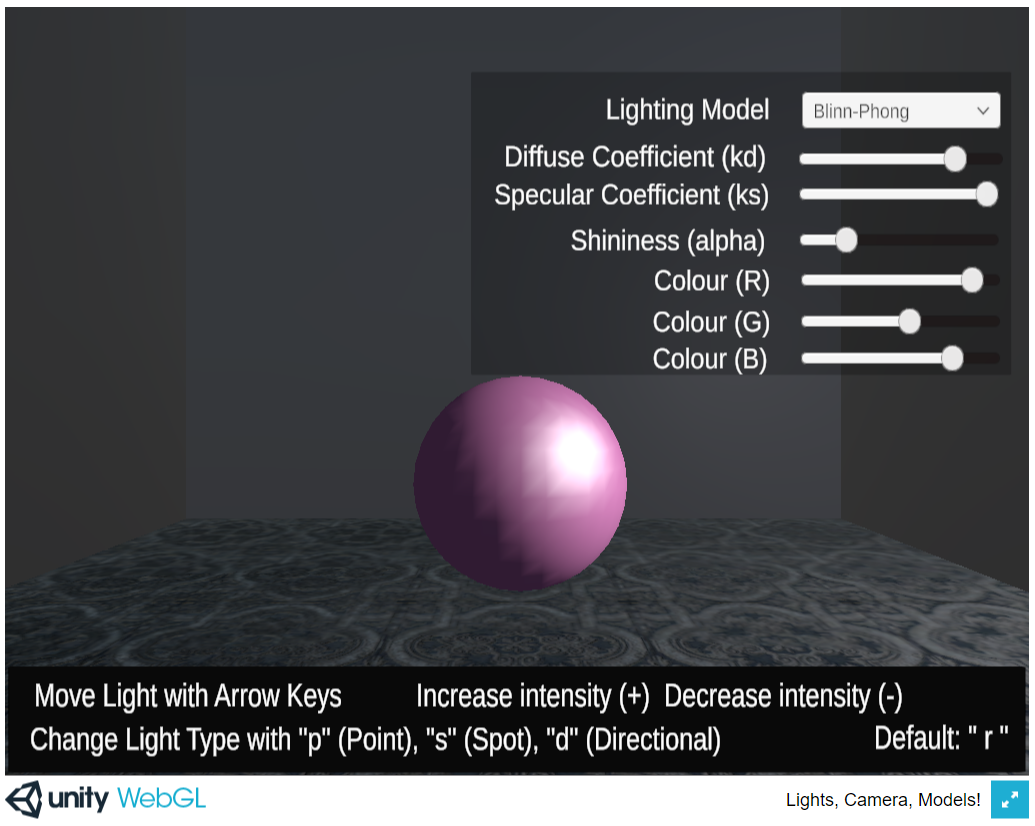
\includegraphics[scale=0.25]{./images/fromVnVPlan/sphere-lit-point-moveBoundsR}
		\caption{Output Variation 2}
		\label{fig:point-bounds-right}
	\end{figure}	
	
	\begin{figure}[h]
		\centering
		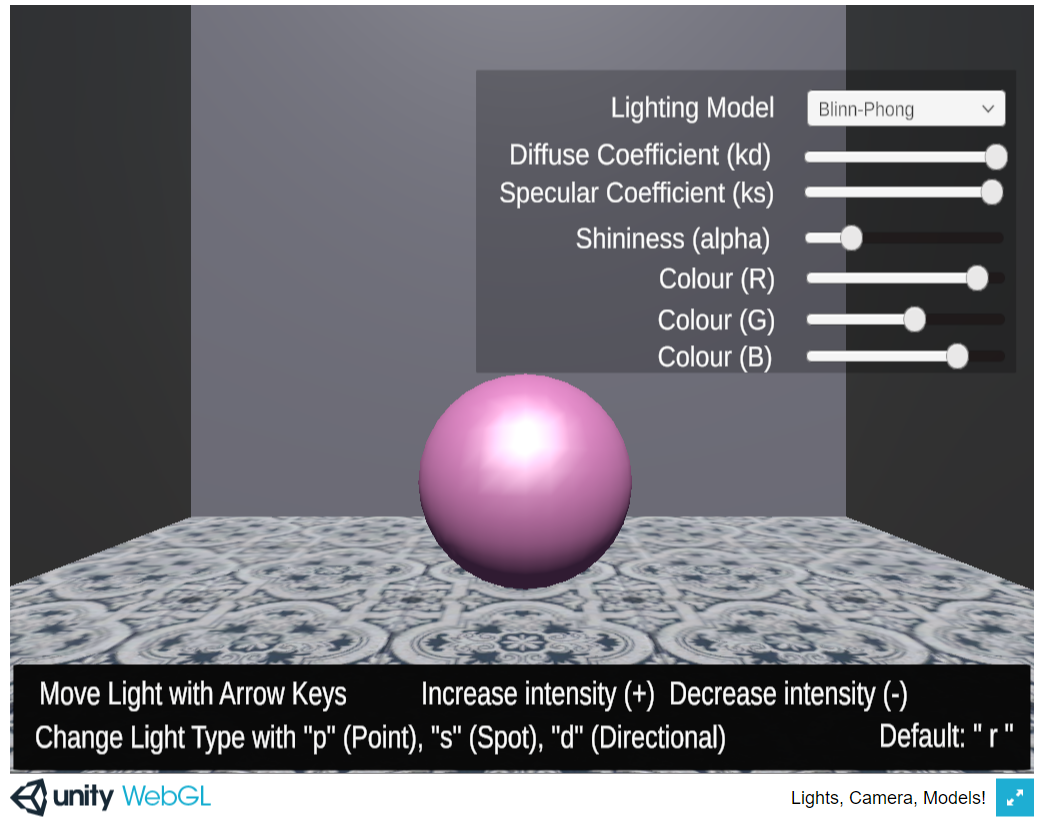
\includegraphics[scale=0.25]{./images/fromVnVPlan/sphere-lit-direction}
		\caption{Output Variation 1}
		\label{fig:directional-bounds-right}
	\end{figure}
	
	\begin{figure}[h]
		\centering
		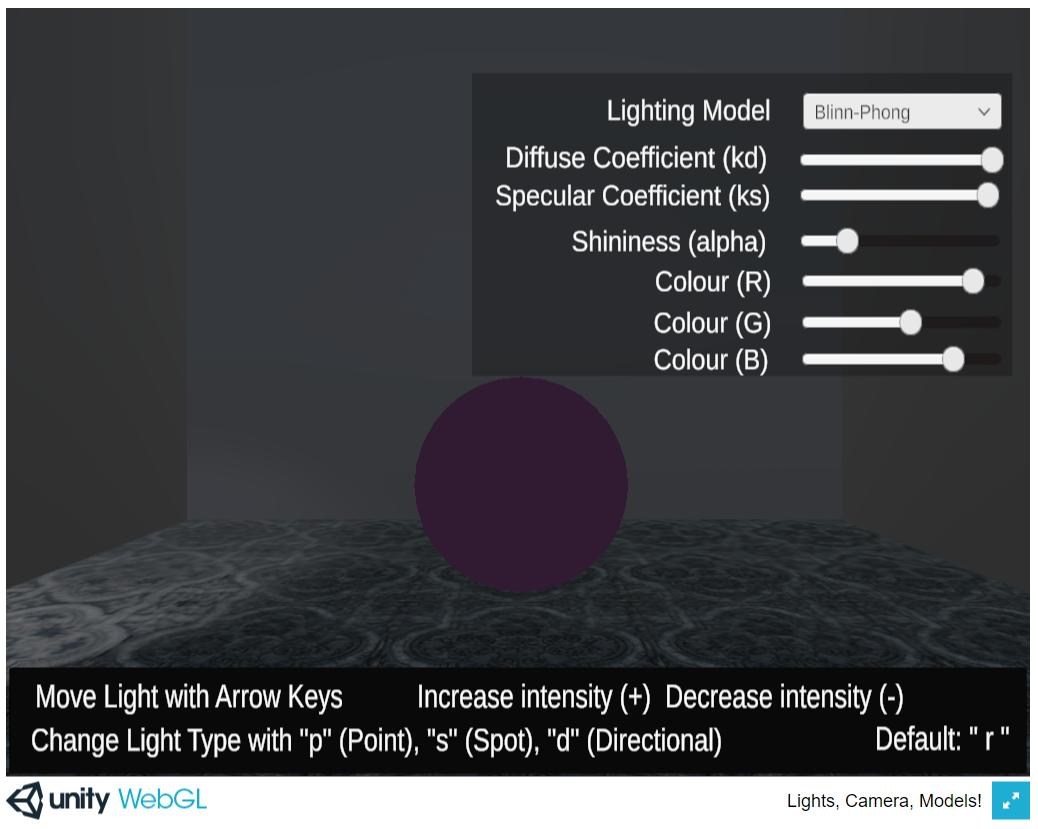
\includegraphics[scale=0.25]{./images/fromVnVPlan/sphere-lit-spotlight-moveBounds}
		\caption{Output Variation 4}
		\label{fig:spotlight-bounds-left}
	\end{figure}	
	
	\begin{figure}[h]
		\centering
		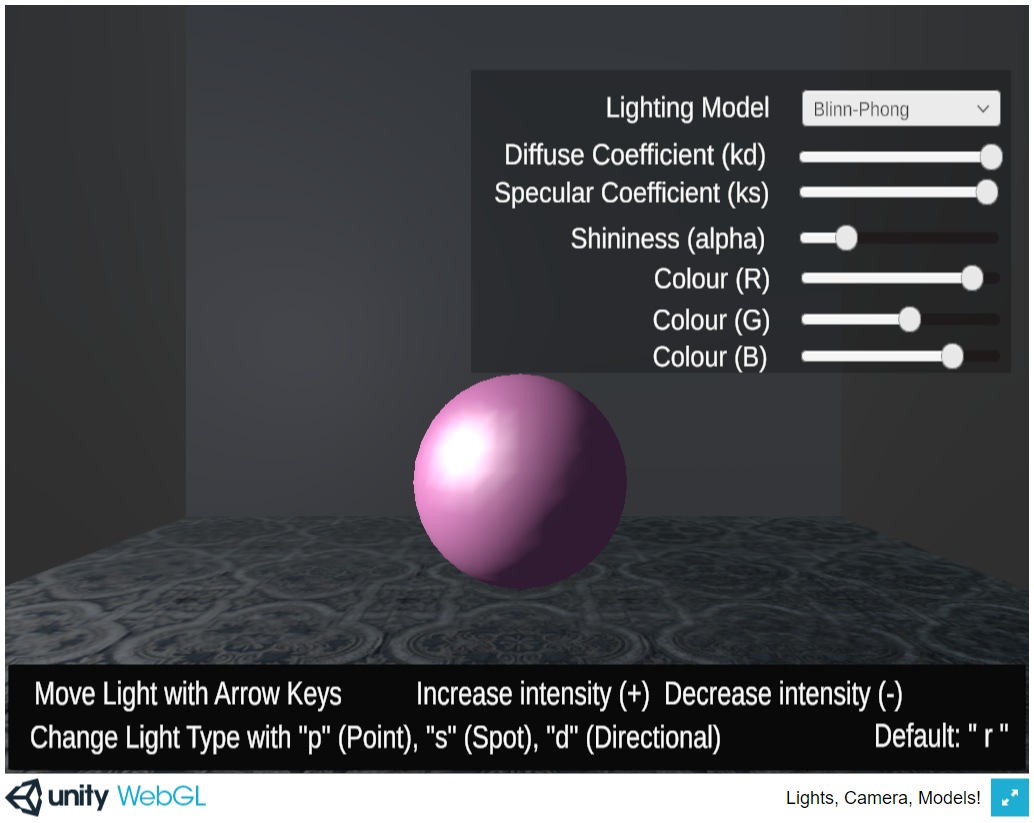
\includegraphics[scale=0.25]{./images/fromVnVPlan/sphere-lit-point-moveBounds}
		\caption{Output Variation 5}
		\label{fig:point-bounds-left}
	\end{figure}	
	
	

	%%Light Type Change	
	\item[\label{test:lightShape}]{lightShape-valid\\}
	
	Control: Manual
	
	Input: \\
	\textit{Variation 1}: Press s\\
	\textit{Variation 2}: Press p\\
	\textit{Variation 3}: Press d\\
	
	Output: Scene render Blinn-Phong lighting model. Intensities and incidence 
	rays are recalculated depending on the type of light source.
	
	\begin{figure}[h]
		\centering
		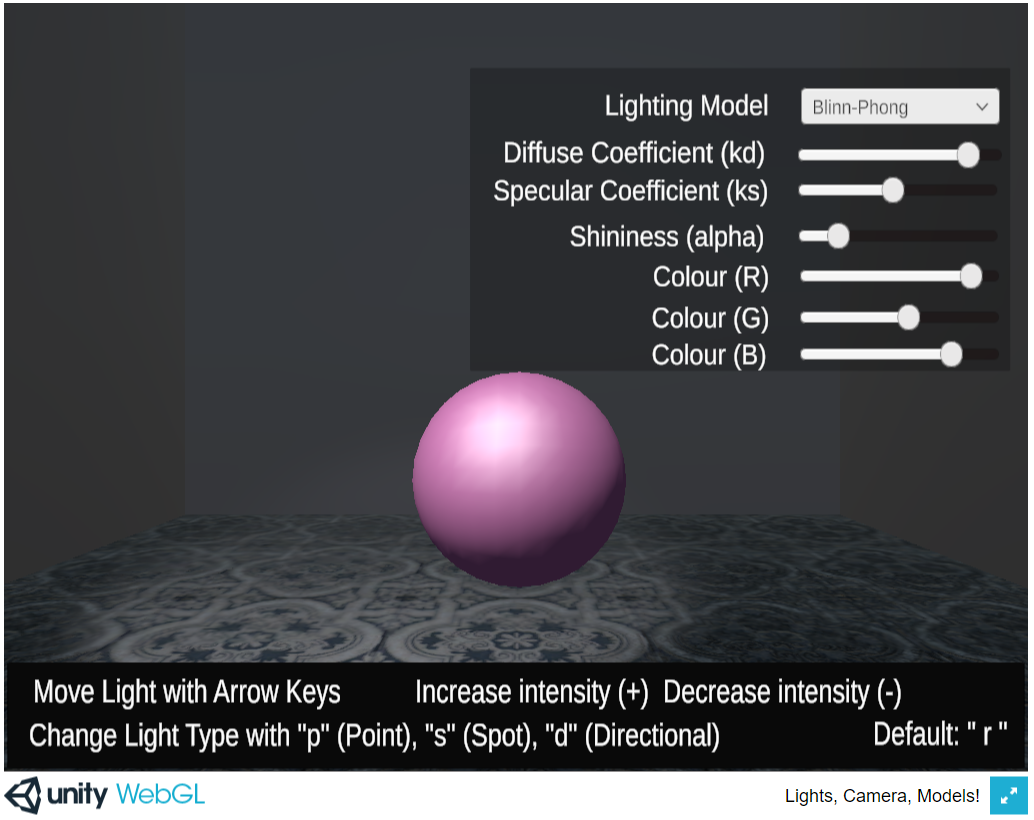
\includegraphics[scale=0.25]{./images/fromVnVPlan/sphere-lit-blinnphong}
		\caption{Output Variation 1}
		\label{fig:spotlight}
	\end{figure}	
	
	\begin{figure}[h]
		\centering
		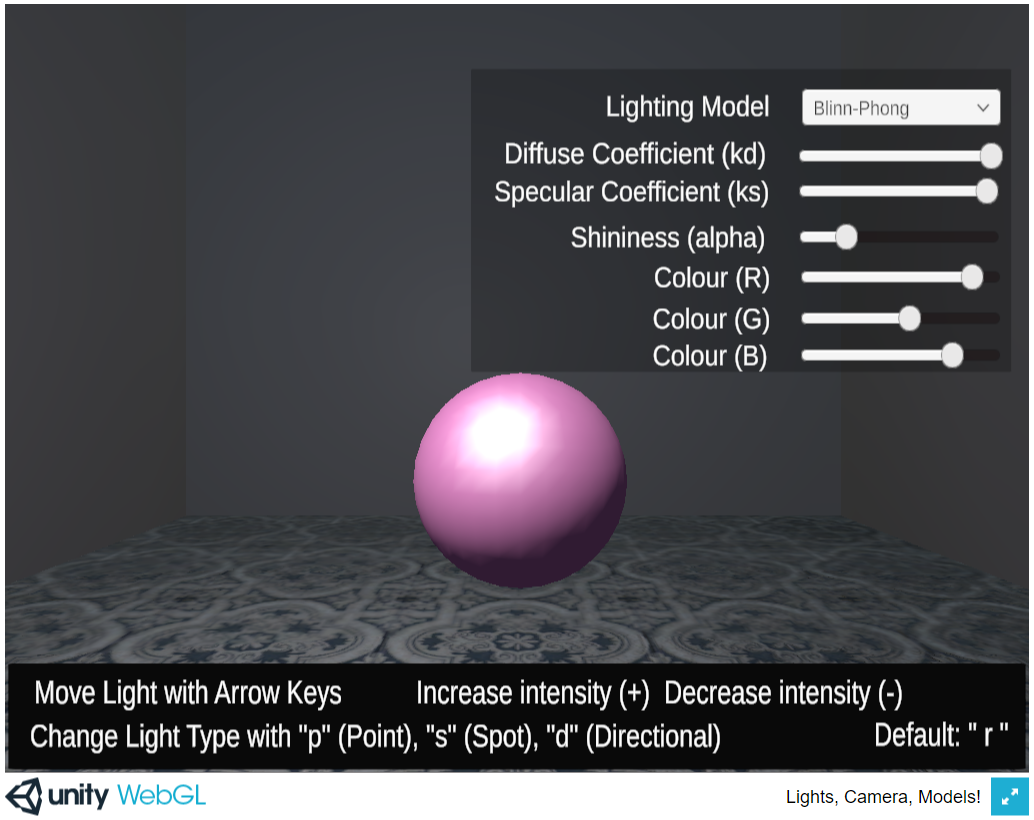
\includegraphics[scale=0.25]{./images/fromVnVPlan/sphere-lit-blinnphong-point}
		\caption{Output Variation 2}
		\label{fig:point}
	\end{figure}	
	
	\begin{figure}[h]
		\centering
		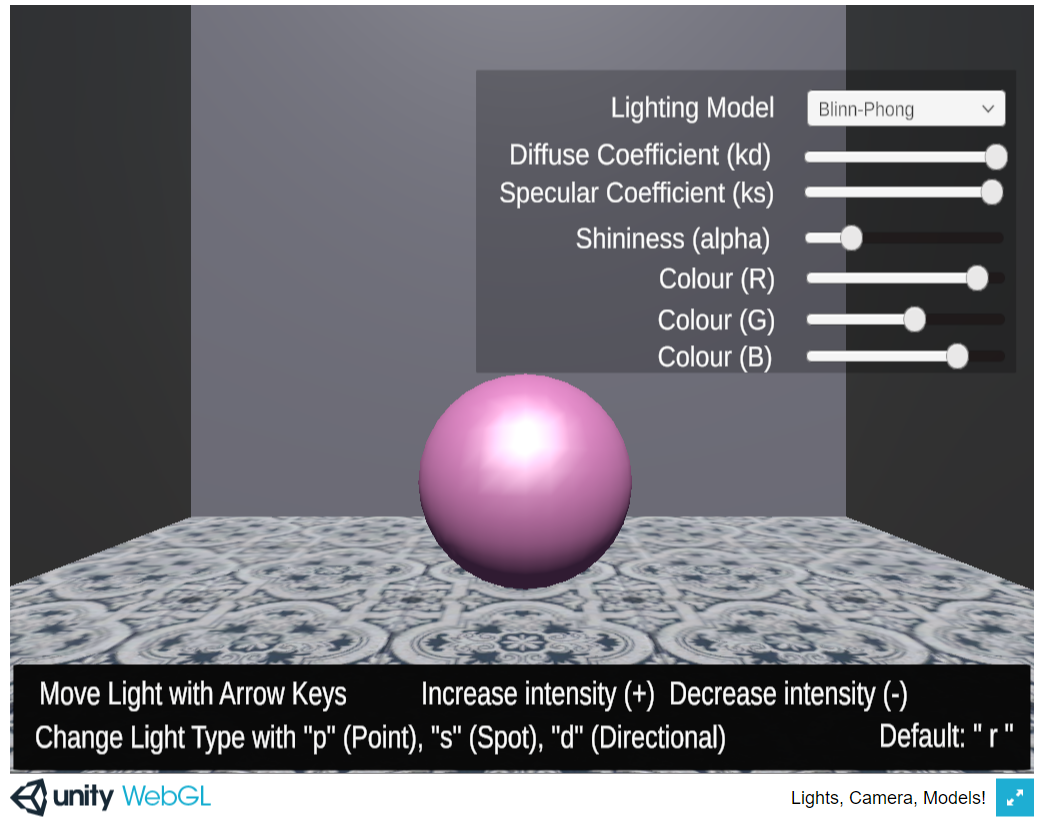
\includegraphics[scale=0.25]{./images/fromVnVPlan/sphere-lit-direction}
		\caption{Output Variation 1}
		\label{fig:directional}
	\end{figure}	
	
	
\end{enumerate}

\section{Nonfunctional Requirements Evaluation}

\subsection{Usability}

\section{Comparison to Existing Implementation}	

This section will not be appropriate for every project.

\section{Unit Testing}

\section{Changes Due to Testing}

\section{Automated Testing}
		
\section{Trace to Requirements}
		
\section{Trace to Modules}		

\section{Code Coverage Metrics}

\bibliographystyle{plainnat}

\bibliography{SRS}

\end{document}